% Options for packages loaded elsewhere
\PassOptionsToPackage{unicode}{hyperref}
\PassOptionsToPackage{hyphens}{url}
%
\documentclass[
]{article}
\usepackage{amsmath,amssymb}
\usepackage{lmodern}
\usepackage{iftex}
\ifPDFTeX
  \usepackage[T1]{fontenc}
  \usepackage[utf8]{inputenc}
  \usepackage{textcomp} % provide euro and other symbols
\else % if luatex or xetex
  \usepackage{unicode-math}
  \defaultfontfeatures{Scale=MatchLowercase}
  \defaultfontfeatures[\rmfamily]{Ligatures=TeX,Scale=1}
\fi
% Use upquote if available, for straight quotes in verbatim environments
\IfFileExists{upquote.sty}{\usepackage{upquote}}{}
\IfFileExists{microtype.sty}{% use microtype if available
  \usepackage[]{microtype}
  \UseMicrotypeSet[protrusion]{basicmath} % disable protrusion for tt fonts
}{}
\makeatletter
\@ifundefined{KOMAClassName}{% if non-KOMA class
  \IfFileExists{parskip.sty}{%
    \usepackage{parskip}
  }{% else
    \setlength{\parindent}{0pt}
    \setlength{\parskip}{6pt plus 2pt minus 1pt}}
}{% if KOMA class
  \KOMAoptions{parskip=half}}
\makeatother
\usepackage{xcolor}
\IfFileExists{xurl.sty}{\usepackage{xurl}}{} % add URL line breaks if available
\IfFileExists{bookmark.sty}{\usepackage{bookmark}}{\usepackage{hyperref}}
\hypersetup{
  hidelinks,
  pdfcreator={LaTeX via pandoc}}
\urlstyle{same} % disable monospaced font for URLs
\usepackage[margin=1in]{geometry}
\usepackage{longtable,booktabs,array}
\usepackage{calc} % for calculating minipage widths
% Correct order of tables after \paragraph or \subparagraph
\usepackage{etoolbox}
\makeatletter
\patchcmd\longtable{\par}{\if@noskipsec\mbox{}\fi\par}{}{}
\makeatother
% Allow footnotes in longtable head/foot
\IfFileExists{footnotehyper.sty}{\usepackage{footnotehyper}}{\usepackage{footnote}}
\makesavenoteenv{longtable}
\usepackage{graphicx}
\makeatletter
\def\maxwidth{\ifdim\Gin@nat@width>\linewidth\linewidth\else\Gin@nat@width\fi}
\def\maxheight{\ifdim\Gin@nat@height>\textheight\textheight\else\Gin@nat@height\fi}
\makeatother
% Scale images if necessary, so that they will not overflow the page
% margins by default, and it is still possible to overwrite the defaults
% using explicit options in \includegraphics[width, height, ...]{}
\setkeys{Gin}{width=\maxwidth,height=\maxheight,keepaspectratio}
% Set default figure placement to htbp
\makeatletter
\def\fps@figure{htbp}
\makeatother
\setlength{\emergencystretch}{3em} % prevent overfull lines
\providecommand{\tightlist}{%
  \setlength{\itemsep}{0pt}\setlength{\parskip}{0pt}}
\setcounter{secnumdepth}{5}
\usepackage{booktabs}
\usepackage{longtable}
\usepackage{array}
\usepackage{multirow}
\usepackage{wrapfig}
\usepackage{float}
\usepackage{colortbl}
\usepackage{pdflscape}
\usepackage{tabu}
\usepackage{threeparttable}
\usepackage{threeparttablex}
\usepackage[normalem]{ulem}
\usepackage{makecell}
\usepackage{xcolor}
\ifLuaTeX
  \usepackage{selnolig}  % disable illegal ligatures
\fi

\author{}
\date{\vspace{-2.5em}}

\begin{document}

\hypertarget{data-analysis}{%
\subsection{Data Analysis}\label{data-analysis}}

Using the MLLT model which allows correlation in the observation errors and underlying cognitive process (OS), we carry out an analysis on the NACC data with the outcomes and predictors of interest as described in (section\_\_\_\_\_\_\_\_\_\_). The Gibb's sampling was repeated 5,000 times with a burn-in of 2,000 samples. Non-informative priors are used for both the linear effects and covariance matrices.

\hypertarget{data-analysis-results}{%
\subsubsection{Data Analysis Results}\label{data-analysis-results}}

\begingroup\fontsize{7}{9}\selectfont

\begin{longtable}[t]{l|l|l|l|l|l}
\hline
  & LOGIMEM & MEMUNITS & DIGIF & DIGIB & TRAILA\\
\hline
time & \cellcolor{white}{-0.06 (-0.26, 0.13)} & \cellcolor{white}{0.01 (-0.20, 0.21)} & \cellcolor{red}{-0.17 (-0.32, -0.02)} & \cellcolor{red}{-0.38 (-0.53, -0.23)} & \cellcolor{red}{-0.28 (-0.49, -0.05)}\\
\hline
RACEWHITE & \cellcolor{red}{-0.27 (-0.43, -0.12)} & \cellcolor{red}{-0.32 (-0.47, -0.15)} & \cellcolor{white}{-0.05 (-0.18, 0.06)} & \cellcolor{white}{0.05 (-0.08, 0.17)} & \cellcolor{white}{-0.10 (-0.28, 0.07)}\\
\hline
SEX & \cellcolor{red}{-0.16 (-0.30, -0.02)} & \cellcolor{red}{-0.23 (-0.38, -0.07)} & \cellcolor{white}{0.08 (-0.02, 0.18)} & \cellcolor{green}{0.10 (0.00, 0.20)} & \cellcolor{white}{0.13 (-0.03, 0.28)}\\
\hline
APOE & \cellcolor{red}{-0.24 (-0.42, -0.05)} & \cellcolor{red}{-0.22 (-0.42, -0.02)} & \cellcolor{white}{0.02 (-0.11, 0.15)} & \cellcolor{green}{0.24 (0.12, 0.37)} & \cellcolor{white}{0.06 (-0.14, 0.25)}\\
\hline
APOESEX & \cellcolor{white}{0.11 (-0.13, 0.36)} & \cellcolor{white}{-0.00 (-0.26, 0.24)} & \cellcolor{white}{-0.08 (-0.25, 0.08)} & \cellcolor{red}{-0.29 (-0.45, -0.12)} & \cellcolor{white}{-0.25 (-0.48, 0.00)}\\
\hline
EDUC & \cellcolor{white}{0.00 (-0.01, 0.01)} & \cellcolor{white}{0.00 (-0.00, 0.01)} & \cellcolor{white}{0.00 (-0.00, 0.01)} & \cellcolor{white}{0.00 (-0.00, 0.01)} & \cellcolor{white}{-0.01 (-0.01, 0.00)}\\
\hline
DEC & \cellcolor{red}{-0.17 (-0.30, -0.05)} & \cellcolor{white}{-0.10 (-0.23, 0.02)} & \cellcolor{red}{-0.12 (-0.24, -0.01)} & \cellcolor{red}{-0.16 (-0.27, -0.05)} & \cellcolor{red}{-0.45 (-0.61, -0.29)}\\
\hline
AgeBase & \cellcolor{red}{-0.01 (-0.02, -0.00)} & \cellcolor{red}{-0.01 (-0.02, -0.01)} & \cellcolor{white}{0.00 (-0.00, 0.01)} & \cellcolor{white}{-0.00 (-0.01, 0.00)} & \cellcolor{red}{-0.02 (-0.02, -0.01)}\\
\hline
\end{longtable}
\endgroup{}

\begingroup\fontsize{7}{9}\selectfont

\begin{longtable}[t]{l|l|l|l|l|l}
\hline
  & TRAILB & WAIS & BOSTON & ANIMALS & VEG\\
\hline
time & \cellcolor{red}{-0.46 (-0.65, -0.25)} & \cellcolor{red}{-0.19 (-0.34, -0.02)} & \cellcolor{white}{-0.06 (-0.28, 0.12)} & \cellcolor{red}{-0.20 (-0.37, -0.02)} & \cellcolor{white}{-0.13 (-0.32, 0.05)}\\
\hline
RACEWHITE & \cellcolor{white}{-0.06 (-0.24, 0.11)} & \cellcolor{red}{-0.24 (-0.36, -0.11)} & \cellcolor{white}{-0.13 (-0.28, 0.02)} & \cellcolor{red}{-0.31 (-0.45, -0.18)} & \cellcolor{red}{-0.30 (-0.44, -0.15)}\\
\hline
SEX & \cellcolor{white}{0.06 (-0.07, 0.19)} & \cellcolor{white}{0.02 (-0.08, 0.12)} & \cellcolor{red}{-0.16 (-0.28, -0.03)} & \cellcolor{white}{-0.08 (-0.20, 0.03)} & \cellcolor{red}{-0.16 (-0.27, -0.05)}\\
\hline
APOE & \cellcolor{white}{-0.05 (-0.23, 0.12)} & \cellcolor{white}{-0.02 (-0.16, 0.10)} & \cellcolor{white}{-0.05 (-0.22, 0.13)} & \cellcolor{white}{-0.11 (-0.27, 0.05)} & \cellcolor{white}{-0.13 (-0.30, 0.03)}\\
\hline
APOESEX & \cellcolor{white}{-0.18 (-0.40, 0.05)} & \cellcolor{white}{-0.15 (-0.31, 0.03)} & \cellcolor{white}{0.04 (-0.19, 0.25)} & \cellcolor{white}{-0.04 (-0.24, 0.17)} & \cellcolor{white}{0.04 (-0.16, 0.25)}\\
\hline
EDUC & \cellcolor{white}{-0.00 (-0.01, 0.00)} & \cellcolor{red}{-0.01 (-0.01, -0.00)} & \cellcolor{white}{-0.00 (-0.01, 0.01)} & \cellcolor{white}{0.00 (-0.01, 0.01)} & \cellcolor{white}{-0.00 (-0.01, 0.00)}\\
\hline
DEC & \cellcolor{red}{-0.27 (-0.41, -0.13)} & \cellcolor{red}{-0.31 (-0.42, -0.22)} & \cellcolor{red}{-0.33 (-0.45, -0.21)} & \cellcolor{red}{-0.14 (-0.26, -0.01)} & \cellcolor{red}{-0.20 (-0.33, -0.08)}\\
\hline
AgeBase & \cellcolor{red}{-0.01 (-0.02, -0.01)} & \cellcolor{red}{-0.01 (-0.02, -0.01)} & \cellcolor{red}{-0.01 (-0.02, -0.00)} & \cellcolor{red}{-0.01 (-0.02, -0.01)} & \cellcolor{red}{-0.01 (-0.02, -0.00)}\\
\hline
\end{longtable}
\endgroup{}

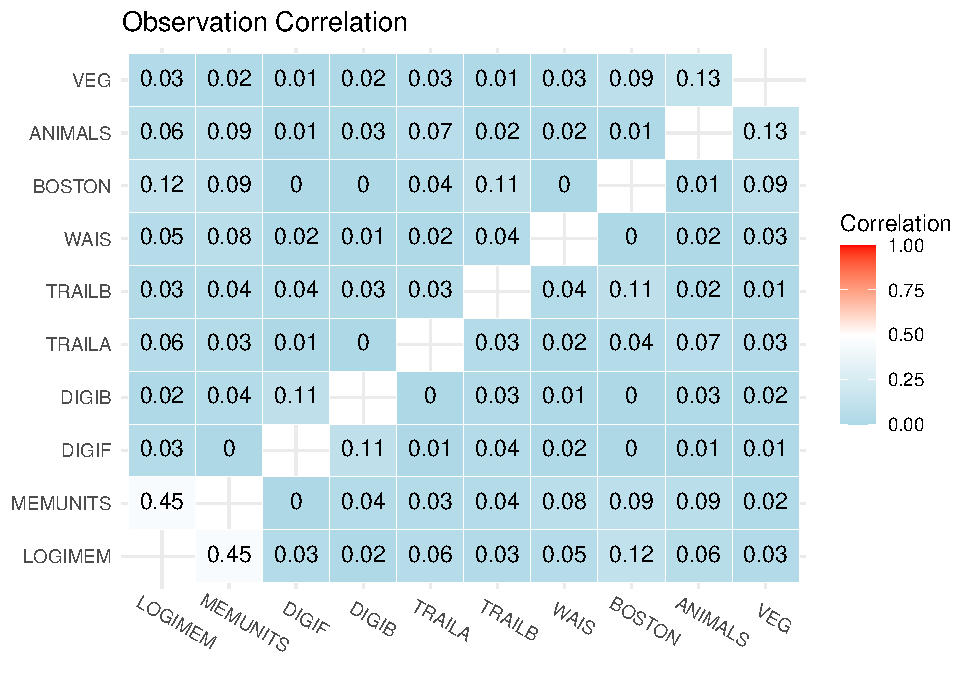
\includegraphics{DataAnalysis_files/figure-latex/unnamed-chunk-3-1.pdf}

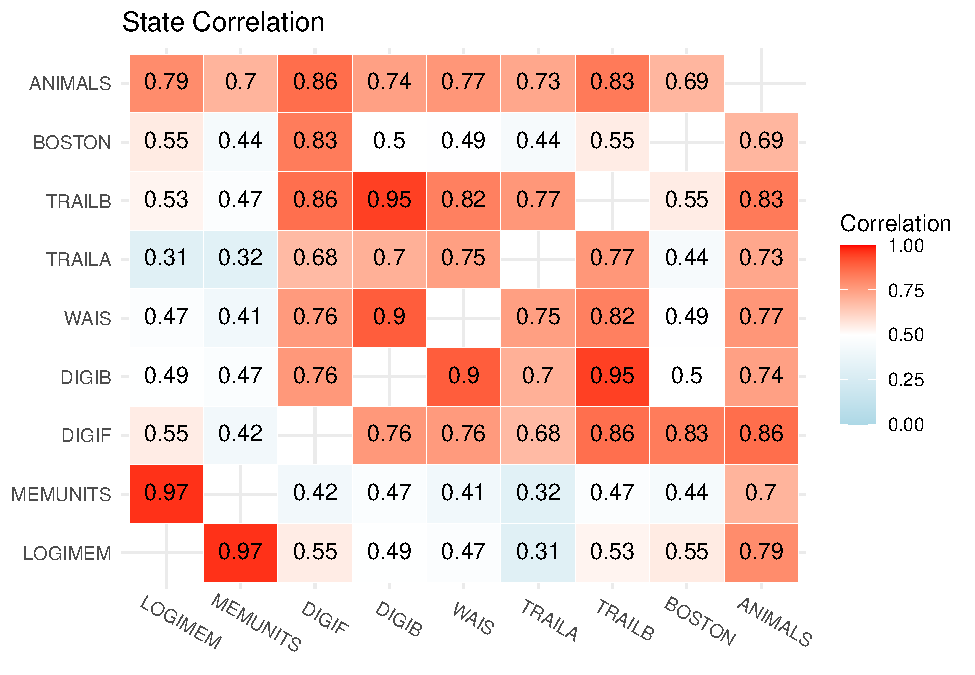
\includegraphics{DataAnalysis_files/figure-latex/unnamed-chunk-4-1.pdf}

\end{document}
